\section{Defining the Edge}
\label{sec:edge}

\enquote{Periphery} is a slippery word. A place can be peripheral because it
is far from where the money is, because it is too small to support its own
specialists and markets, or because it is politically marginal. These
overlap, but they are not the same, and conflating them is how arguments
about remoteness go wrong. This paper uses two separate, measurable
dimensions.

\paragraph{Remoteness.} \emph{Economic remoteness} is the average distance
from a country to the rest of the world's output, with each partner weighted
by its share of world GDP (\cref{app:data}). It is in the spirit of the
market-access measures of \textcite{redding2004}: what matters is not
kilometres to the nearest coast but kilometres to customers, suppliers and
capital. Distances come from CEPII's GeoDist database \parencite{mayer2011};
GDP is the \windowStart--\windowEnd{} average from the World Bank. The median
economy sits \remoteMedianKm{} km from world output. \remoteMinName{} is the
least remote at \remoteMinKm{} km, \remoteMaxName{} the most at
\remoteMaxKm{} km. Tonga, at \remoteTongaKm{} km, ranks
\remoteTongaRank{} of \nCountriesRemote{} economies by remoteness; the
median Pacific island state is \remotePacificMedianKm{} km away.

\paragraph{Scale.} \emph{Scale} is simply population. The UN lists
\nSIDSunList{} Small Island Developing States (SIDS) and \nLLDC{} Landlocked
Developing Countries \parencite{unm49}; \nSIDS{} of the SIDS appear in the
World Bank's data. The median island state has \popSIDSMedianK{} thousand
people, and \shareSIDSUnderOneM\% have fewer than a million.

\begin{figure}[t]
  \centering
  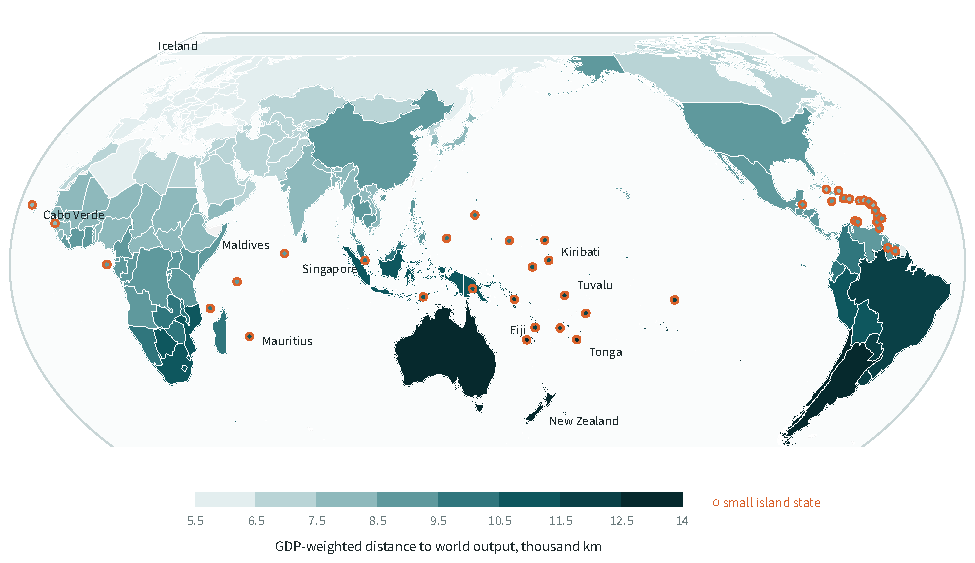
\includegraphics[width=\linewidth]{../figures/remoteness_map.pdf}
  \caption{\takeaway{The Pacific is the far edge of the world economy.}
    Economic remoteness: the GDP-weighted average distance from each economy to
    the rest of world output, \windowStart--\windowEnd. Small island states are
    shown as dots.
    \source{CEPII GeoDist \parencite{mayer2011}; World Bank WDI; UN M49 SIDS list.
    Map: Natural Earth.}}
  \label{fig:map}
\end{figure}


The first finding is that the two dimensions really are distinct. Across
countries the correlation between log remoteness and log population is just
\corrRemotePop. \Cref{fig:map} shows why. The far edge of the world economy is
the South Pacific, together with Australia, New Zealand and the Southern Cone
of Latin America. Several of the archetypal \enquote{peripheral} success stories
are not remote at all on this measure: Iceland (\remoteIcelandKm{} km) and
the Faroe Islands (\remoteFaroesKm{} km) sit between Europe and North America
and are among the \emph{least} remote places on Earth. They are small, not
far. Singapore (\remoteSingaporeKm{} km) and Mauritius (\remoteMauritiusKm{}
km) are moderately remote. This matters for \cref{sec:escape}.

\paragraph{Far versus small.} Which handicap costs more? \Cref{tab:regression}
regresses log income per head (PPP) on log remoteness and log population. On
its own, remoteness has a large negative association with income. Adding
government effectiveness, a crude proxy for institutions, roughly halves the
remoteness coefficient but leaves it large and precisely estimated: holding
governance constant, doubling remoteness is associated with
\regDoubleRemotePctAbs\% lower income per head. Population, by contrast, has a
small coefficient (\regPopTwo{} in column 2); being tiny is not, by itself,
associated with being poor---echoing \textcite{easterly2000}. Being landlocked
carries an extra penalty of about \regLLDCpct\%, consistent with
\textcite{limao2001}. Once distance and governance are accounted for, being a
small island adds nothing significant (\regSIDS, s.e.\ \regSIDSse).

\begin{table}[t]
\centering
\caption{\takeaway{Distance, not size, carries the income penalty.} OLS of log$_{10}$
  GDP per capita (PPP, \windowStart--\windowEnd) on log$_{10}$ remoteness and
  log$_{10}$ population. Robust (HC1) standard errors in parentheses;
  $^{*}p<0.1$, $^{**}p<0.05$, $^{***}p<0.01$.}
\label{tab:regression}
\small\sffamily
% generated by scripts/export_stats.py
\begin{tabular}{@{}lccc@{}}
\toprule
 & (1) & (2) & (3) \\
\midrule
log remoteness & $-2.25^{***}$ & $-1.11^{***}$ & $-1.05^{***}$ \\
 & $(0.35)$ & $(0.18)$ & $(0.21)$ \\[2pt]
log population & $-0.11^{***}$ & $-0.04^{**}$ & $-0.05^{**}$ \\
 & $(0.03)$ & $(0.02)$ & $(0.02)$ \\[2pt]
Government effectiveness &  & $0.41^{***}$ & $0.38^{***}$ \\
 &  & $(0.02)$ & $(0.02)$ \\[2pt]
SIDS &  &  & $-0.07$ \\
 &  &  & $(0.07)$ \\[2pt]
Landlocked (LLDC) &  &  & $-0.19^{***}$ \\
 &  &  & $(0.06)$ \\[2pt]
Constant & $13.71^{***}$ & $8.74^{***}$ & $8.65^{***}$ \\
 & $(1.42)$ & $(0.75)$ & $(0.79)$ \\[2pt]
\midrule
Countries & 197 & 193 & 193 \\
$R^2$ & 0.22 & 0.73 & 0.74 \\
\bottomrule
\end{tabular}

\source{World Bank WDI and WGI; CEPII; author's calculations.}
\end{table}

These are associations, not causal estimates. Governance is itself partly an
outcome of geography and history, so controlling for it may absorb some of
remoteness's true effect, while omitted factors---colonial history above
all \parencite{acemoglu2001}, but also natural resources and language---may
inflate it. The point of \cref{tab:regression} is narrower: in the cross-section,
the burden of the edge loads on \emph{distance}, and the remedies for distance
(connectivity, redundancy, pooled logistics) differ from the remedies for
smallness (pooled institutions, shared services).
